\section{Benchmarks}
The final version of the \textit{Mosaico} software has been tested for performance on the actual Raspberry Pi hardware, focusing on both CPU and memory usage. These tests yielded satisfactory results, especially considering the hardware limitations of the Raspberry Pi Zero.

\subsection{CPU Usage}

The CPU performance was measured across various scenarios, ranging from idle states (with no widgets displayed) to the execution of the most complex widget available. As shown in the figure below, the CPU usage started at approximately 60\% when no widgets were active, increasing to nearly 80\% when displaying the most demanding widget.

\begin{figure}[H]
    \centering
    \begin{minipage}[b]{0.98\textwidth}
        \centering
        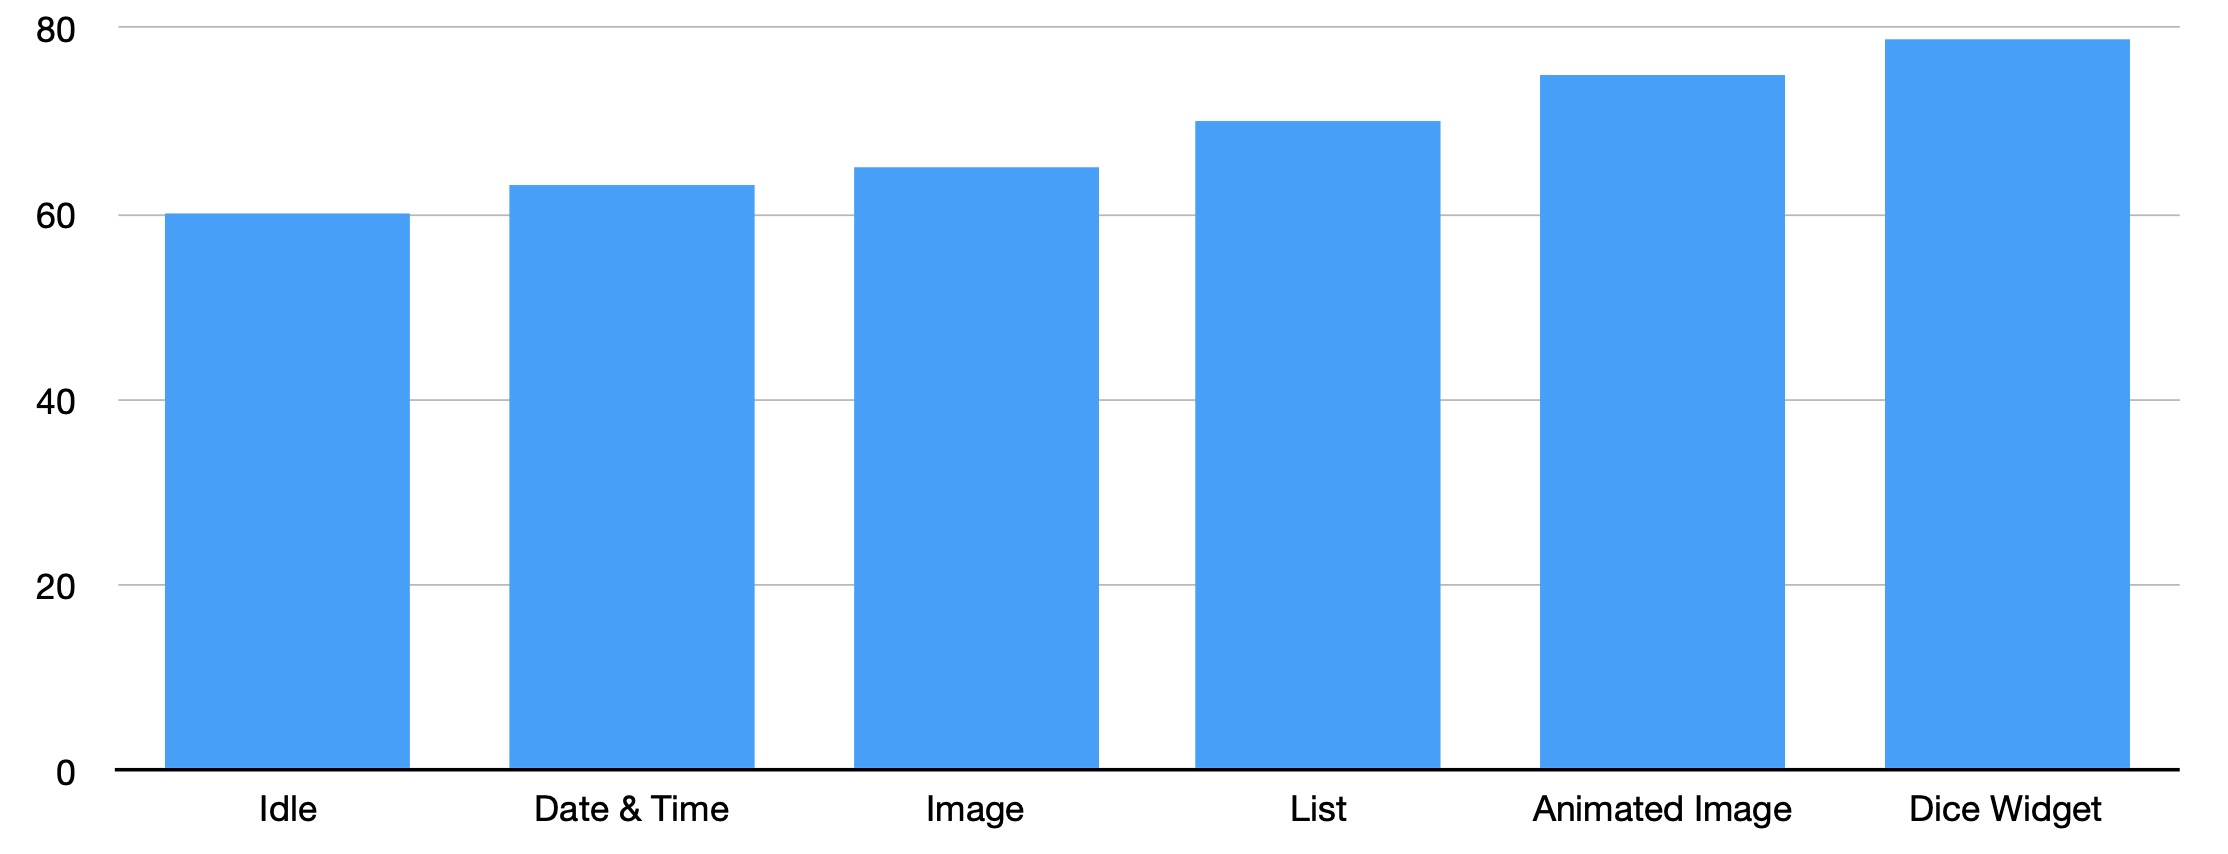
\includegraphics[width=\textwidth]{tesi/img/benchmarks/CPU.png}
        \caption*{CPU performance on a Raspberry Pi Zero (Single Core 1GHz)}
    \end{minipage}
\end{figure}

These results are particularly noteworthy considering the Raspberry Pi Zero operates with a single-core 1GHz processor. Despite these hardware constraints, \textit{Mosaico} demonstrates a considerable degree of efficiency, with room for further optimization. This provides confidence that even more complex widgets can be handled with only marginal increases in CPU load.


\subsection{Memory Usage}
Memory consumption was another key area of focus during performance testing. The use of a lightweight operating system, such as DietPi, proved to be a wise choice, as it minimized the overall system resource usage while maintaining sufficient memory for the app's modules to function efficiently.

\begin{figure}[H]
    \centering
    \begin{minipage}[b]{0.32\textwidth}
        I achieved excellent results even regarding RAM usage, with both my app modules occupiyng only about 15\% of the total system memory while DietPI allowed to run using only about 17\% of total system usage. Remember that the Raspberry Pi Zero has only about 477Mb of usable memory so my software used about 70Mb of memory.
    \end{minipage}
    \begin{minipage}[b]{0.65\textwidth}
        \centering
        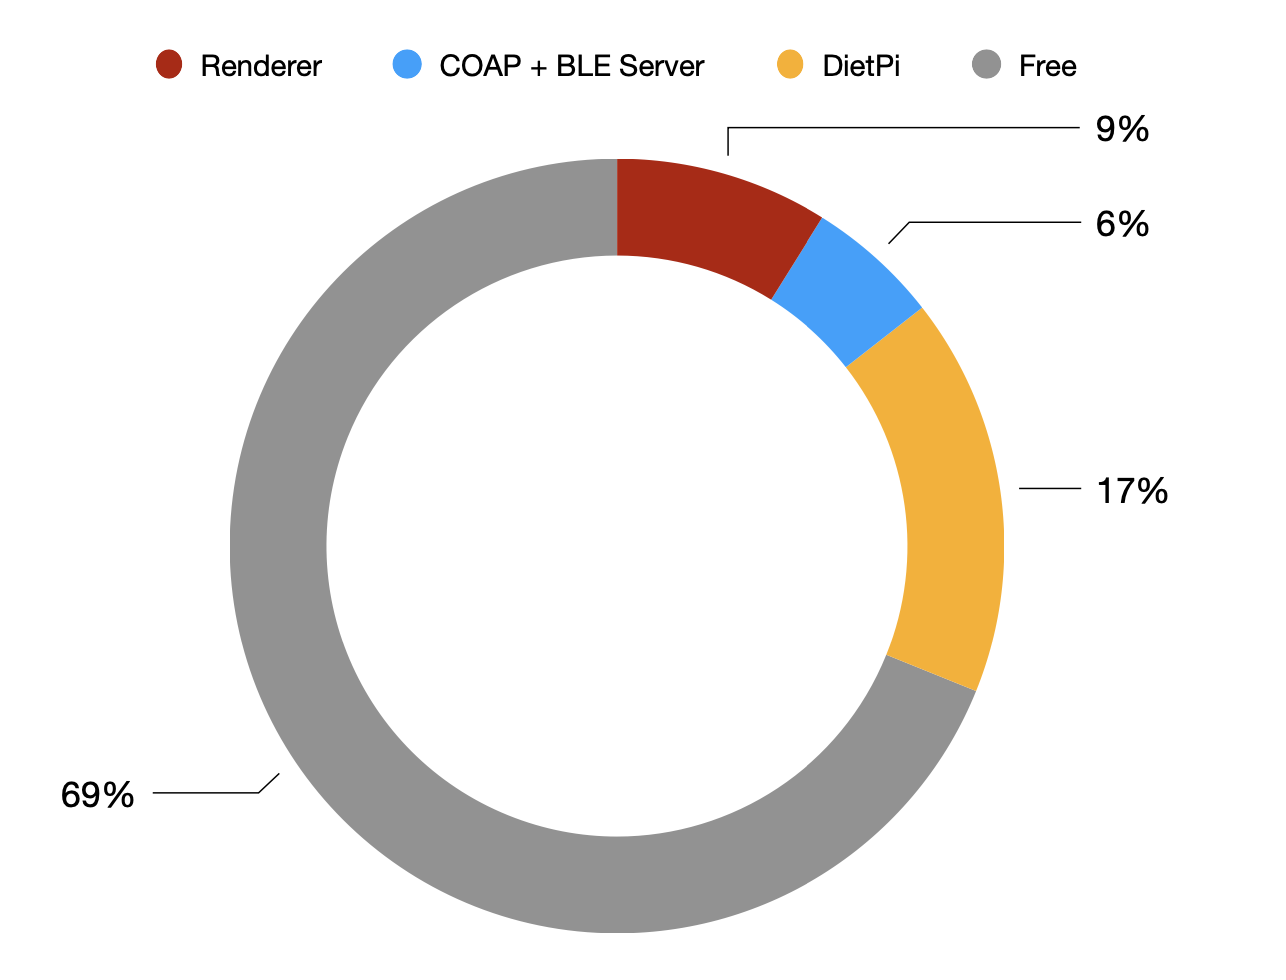
\includegraphics[width=\textwidth]{tesi/img/benchmarks/RAM.png}
        \caption*{System RAM utilization}
    \end{minipage}
\end{figure}

\subsection{Conclusion}

The performance benchmarks highlight that \textit{Mosaico} runs efficiently on a minimal system setup like the Raspberry Pi Zero, utilizing only a modest portion of CPU and memory resources. This efficiency allows for a seamless user experience without overburdening the hardware, and it opens the door for future optimizations that can further improve performance. These findings underscore the app's capability to run effectively even on low-powered devices, making it accessible to a wider range of users.
\newpage
\section{Latency}
\subsection{Protocol Performance: CoAP}

In assessing the overall responsiveness and snappiness of the \textit{Mosaico} app, one of the primary metrics evaluated was the performance of the Constrained Application Protocol (CoAP), which is the key communication protocol used to control the matrix features. Given the constrained environment in which the system operates, particularly on a Raspberry Pi Zero, it was crucial to determine how well CoAP could handle request processing and data transfer between system components.

The results of the testing were highly satisfactory. As predicted, CoAP demonstrated excellent performance, with the majority of basic requests—such as activating, stopping, or switching widgets—being processed in approximately 100 milliseconds. This level of efficiency is particularly impressive when considering the hardware limitations. The minimal latency observed during the testing indicates that CoAP is well-suited for real-time interactions between the app and the matrix device, ensuring a smooth user experience even under constrained conditions.

\begin{center}
  \makebox[\textwidth]{
  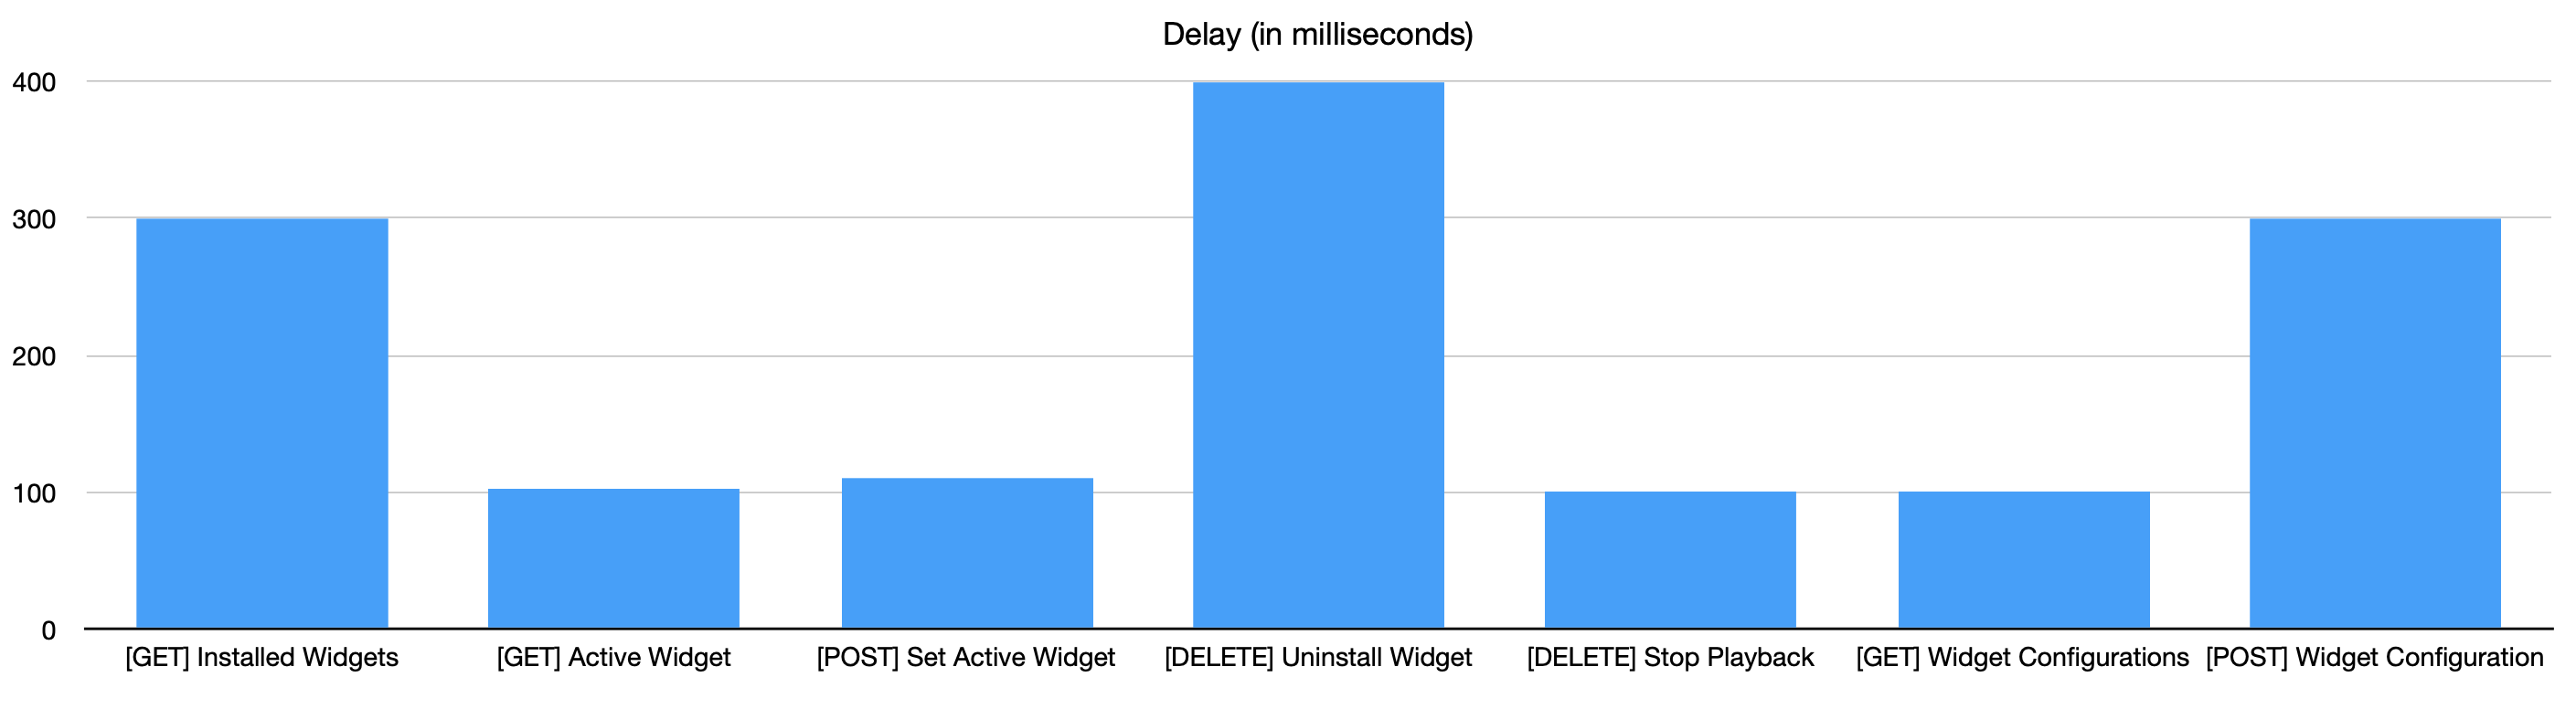
\includegraphics[width=0.8\paperwidth]{tesi/img/benchmarks/COAP.png}}
\end{center}

One notable exception to the generally fast performance was the installation of new widgets from the app's store, which took approximately 8 seconds. This longer duration can be attributed to two main factors: the need to download files from an external Git repository and the relatively slow storage access speeds of the Raspberry Pi Zero. While this delay is understandable, particularly in a resource-constrained environment, it highlights an area for potential optimization in future iterations of the system.

CoAP proved to be an efficient and reliable protocol for managing communication between the app and the matrix device, delivering swift responses in most use cases while leaving room for improvement in more resource-intensive operations like widget installations.


\section{User Feedback}

User feedback has played a pivotal role in refining \textit{Mosaico}, especially given the project's complexity and its reliance on hardware that might not be readily available to all testers. To address this, I developed web simulators \ref{web-simulator} that allowed users to interact with the app in a virtual environment, greatly expanding the range of people able to provide feedback.

Testers identified several key areas for improvement, including both functional bugs and UI/UX enhancements. For example, some users pointed out issues such as notification stacking, where notifications could overlap in an unintuitive way. This feedback was instrumental in identifying and resolving the problem before the official release.

Moreover, several testers suggested improvements for transitions between widgets, which have now been implemented to create a smoother, more visually appealing experience. Others noted that adding additional widget features, such as previews of fonts or new widgets ideas.

Overall, the feedback provided by early testers has been invaluable in refining the app and ensuring that \textit{Mosaico} is more intuitive, stable, and feature-rich for all users.


\section{Deployment} Perhaps one of the least glamorous but most critical aspects of software development is the deployment process. Transitioning the entire project, along with its various dependencies, to a new machine can be both technically challenging and time-consuming. Ensuring that the development environment mirrors the production environment is essential for a seamless deployment, but achieving this can often be fraught with difficulties.

Fortunately, over the past few years, I have been utilizing Docker, which has drastically streamlined my development and deployment processes. Docker enables the creation of isolated, containerized environments that replicate the production environment with minimal overhead. This ensures consistency between local development and live deployment, significantly reducing the likelihood of environment-specific issues. For this project, I employed a set of custom scripts to dockerize the Laravel application\footnote{\url{https://github.com/codexdevelopment-it/dockerized-laravel}}, alongside all required services such as the database and proxy, to get the entire application up and running smoothly.

\subsection{Self-Hosting} A relatively recent but highly rewarding endeavor I embarked upon is self-hosting. About a year ago, I ventured into this fascinating domain, purchasing a dedicated server to host all my internal and public services, thereby eliminating the need to rely on external VPS providers. Self-hosting not only grants full control over the infrastructure but also reduces long-term operational costs, as I am no longer paying recurring fees to third-party hosting providers.

The server's infrastructure is virtualized using Proxmox\footnote{\url{https://www.proxmox.com/}}, a robust, open-source platform for enterprise-level virtualization. Proxmox's comprehensive feature set includes a web-based interface that simplifies the management of virtual machines (VMs), containers, software-defined storage, and networking. This has greatly enhanced my ability to manage complex projects and services efficiently.

When deploying a new project, I simply create a new Linux Container (LXC) with Docker support, clone the repository, and execute a predefined bash script to initiate the deployment process. The entire system is up and running in minutes. Additionally, I configure a new subdomain for the project and use a reverse proxy with automatic HTTPS support\footnote{\url{https://caddyserver.com/}} to direct traffic to the corresponding container. One of the key advantages of this setup is the ease with which I can manage backups—thanks to Proxmox's virtualized storage volumes, I can create incremental backups of entire disks rather than backing up individual files, significantly simplifying the backup and restore process.

This self-hosting infrastructure has provided me with a highly flexible, cost-effective, and scalable environment in which I can develop, deploy, and manage my projects with ease.

\subsection{AppStore and PlayStore}
Publishing the application on both the Apple App Store and Google Play Store was a pivotal moment in making my project accessible to a broad audience. Since I used Flutter as the core development framework, the cross-platform compatibility significantly simplified the process of handling Android fragmentation. With Flutter, I was able to write a single codebase that worked seamlessly across both platforms, ensuring that the user experience was consistent and smooth on various devices.

The app only requires Bluetooth and photo access, both of which are essential for configuring the LED matrix widgets. Bluetooth is used for connecting to the matrix device, while photo access allows users to upload images for specific widgets. Beyond these two permissions, the project has a strict policy against data collection or remote storage. Staying true to the open-source philosophy, the app does not collect or store user data in any remote database, offering users more control and privacy. This adherence to privacy meant that the often tedious privacy approval process became much smoother, as there was no sensitive data being transferred or stored, allowing for a quicker review.

Being fully open-source further reinforces the transparency of the application. Users can inspect the code, ensuring that no hidden data collection mechanisms exist, which adds trust and aligns with the core values of user empowerment and privacy.